%\chapter{Processing and Manufacturing}
\setlength{\headheight}{12.71342pt}
\addtolength{\topmargin}{-0.71342pt}

\section{Processing and Manufacturing}
The production process of the protein bar can be seen on Figure 7.
\begin{figure}[H]
    \centering
    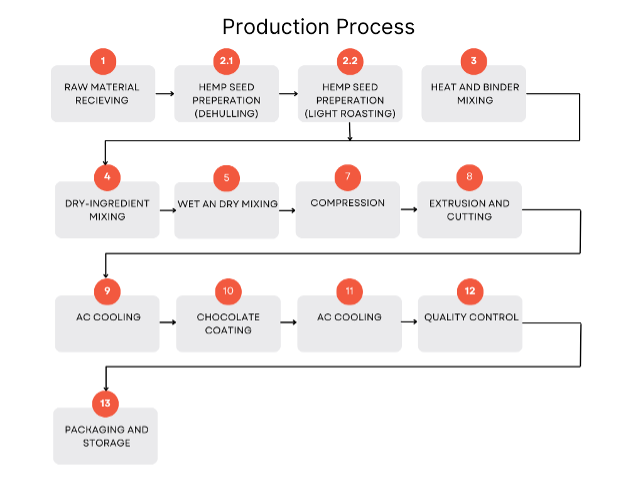
\includegraphics[width=0.8\textwidth]{Figures/fig_process_01.png}
    \caption{A flowchart with a visualization of the production process of the hemp protein bar}
    \label{fig:process_flow_diagram}
\end{figure}

\textit{Sourcing and preparing} raw materials – all ingredients are inspected for quality and stored under appropriate conditions to maintain freshness. All ingredients are weighed and portioned accurately according to the recipe formulation, ensuring batch-to-batch uniformity. This ensures that only safe, high-quality, and properly measured ingredients enter the mixing stage, laying the foundation for a consistent protein bar in terms of flavor, texture, and nutritional profile.

\vspace{1em}
\textit{Dehulling hemp seed} – Increases absorption of proteins and nutrients.

\vspace{1em}
\textit{Light roasting} – of the dehulled hemp seed (75°C-80°C) - improves digestibility, and reduces anti-nutritional factors and lower microbial load.

\vspace{1em}
\textit{Mixing} to homogeneous mixture – evenly distributed throughout the mixture providing a consistent texture and flavor in every bar. Time and temperature in mixing are controlled to ensure that every batch is consistent.

\vspace{1em}
\textit{Compression} – shaping the mixture into a form that is suitable for further processing. Using large presses ensures a uniform sheet, which helps create consistency in texture and flavor throughout the bar.

\vspace{1em}
Extrusion and cutting – A combination of extrusion and cutting technologies are used to shape the mixtures into bars. The extrusion process forces the mixture through a die, after which a knife cuts the long bars into the desired length.

\vspace{1em}
AC cooling – is used to ensure that the bar maintains the desired temperature throughout the process, as mixing and pressure from extrusion can increase the temperature of the product.

\vspace{1em}
Chocolate coating – for flavour.

\vspace{1em}
\textit{AC cooling} – to solidify the chocolate.

\vspace{1em}
\textit{Quality control} – Both automated sensors and visual inspection for defects or foreign objects. Taking samples to ensure that our product meets quality standards, as well as for example checking that the product contains enough protein to be claimed as a product with a high protein content. 

\vspace{1em}
\textit{Packaging} – wrap each bar individually and in a material that keeps the protein bar safe and to ensure that the bar does not undergo oxygenation and to preserve freshness. This process also includes labelling and coding to ensure traceability and compliance with regulatory requirements.

\subsection{Effects on Processing}
Hemp seeds contain several antinutritional, such as phytic acid, tannins and saponins. The presence of tannins and saponins can reduce the bioavailability of nutrients and disrupt both metabolism and digestive functions (kapitel 4 hampbog). The presence of phytic acid can lead to mineral deficiencies (e.g. iron, zinc and calcium), as it can inhibit the absorption of these. (kapitel 10 hampbog). Polyphenols, of which tannins are a part, are often found in the shell of hemp seeds (hemp nutritional value pdf). The same applies to phytic acid. Studies have shown that there is significantly more phytic acid present in whole hemp seeds 3.5 g/100g compared to 2.1 g/100g in hulled hemp seeds. That is a reduction of 40\%. (kapitel 4 hampbog).

\vspace{1em}
According to House et al. (2010), whole hemp seeds have a protein digestibility of approximately 84–86\% and a protein digestibility-corrected amino acid score (PDCAAS) value of 49–53\%, while dehulled hemp seeds reach a digestibility of 91–97\% and a PDCAAS value of 63–66\%. This improvement is primarily due to the fact that the hull contains a large part of the fiber fraction of the seed, which inhibits digestibility, so when the hull is removed, the fiber content is significantly reduced, making the protein more available and thus improving the overall protein assessment (PDCAAS) (Evaluating the Quality of Protein from Hemp Seed pdf.) Therefore, by using a majority of dehulled hemp seeds instead of whole hemp seeds, we reduce the content of antinutrients and increase the nutritional quality of the protein.

\vspace{1em}
Plant proteins naturally contain antinutritional factors such as trypsin inhibitors, glucosinolates, phenols and phytates, together with a high content of dietary fiber, which can negatively affect protein and amino acid digestibility and bioavailability. Heat processing can effectively help to remove or reduce these compounds, leading to higher protein digestibility. However, high heat treatment can have negative effects as it can affect the chemical transformations of amino acids. Some amino acids, such as lysine, can be chemically transformed and become unavailable during heat treatment or other severe processes, leading to problems such as the formation of Maillard reaction products. This underlines the need for appropriate processing conditions to avoid such. (Protein Quality Report No 92 web version .pdf)



\begin{table}[h]
    \centering
    \caption{Protein digestibility-corrected amino acid scores of hemp protein sources in comparison to other food proteins. (Evaluating the Quality of Protein from Hemp Seed pdf.)}
    \label{tab:process_table_01}
    \begin{tabular}{l c}
    \hline
    \textbf{Protein source} & \textbf{PDCAAS (\%)} \\
    \hline
    Casein               & 100 \\
    Egg white            & 100 \\
    Beef                 & 92  \\
    Soy protein isolate  & 92  \\
    Chickpeas (canned)   & 71  \\
    Pea flour            & 69  \\
    Kidney beans (canned)& 68  \\
    Dehulled hemp seed   & 61  \\
    Pinto beans (canned) & 57  \\
    Rolled oats          & 57  \\
    Lentils (canned)     & 52  \\
    Hemp seed            & 51  \\
    Hemp seed meal       & 48  \\
    Whole wheat          & 40  \\
    Almond               & 23  \\
    \hline
    \end{tabular}
\end{table}

\vspace{1em}
At the same time, a study has shown that hemp protein isolates improved proteolysis when heated at 75 °C and 80 °C, but already at 90 °C it caused reduced proteolysis. (hemp seed bioactivity pdf) Therefore, we have chosen to lightly roast our dehulled hemp seeds to achieve the highest possible protein absorption, but with an eye not to reach too high a temperature, as we want to avoid a greater loss of lysine and reduced proteolysis.

